\documentclass{sciposter}
\usepackage{lipsum}
\usepackage{listings}
\usepackage{epsfig}
\usepackage{amsmath}
\usepackage{amssymb}
\usepackage{multicol}
\usepackage{graphicx,url}
\usepackage[portuges, brazil]{babel}   
\usepackage[utf8]{inputenc}

\newtheorem{Def}{Definition}


\title{Projeto Interativo III\\ Angry Robots}


\author{Caroline Bomfim do Espirito Santo, Mahaira Soares de Souza, Rafael da Silva Santos, Thiago de Sousa Messias}


\institute 
{Bacharelado em Ciência da Computação\\
Centro Universitário SENAC - Campus Santo Amaro
(SENAC-SP)\\
Av. Engenheiro Eusébio Stevaux, 823 -- Santo Amaro, São Paulo -- CEP 04696-000 -- SP -- Brasil}


\email{caroline.bomfim@hotmail.com.br, mahaira\_souza@hotmail.com, rafa\_silva.santos@hotmail.com, messiasthi@gmail.com}

\leftlogo[1]{Senac-logo}
\rightlogo[2]{bcc-logo}

\begin{document}

\conference{{\bf PI III}- Senac, 05 de Maio de 2014, São Paulo, Brasil}

\maketitle

\begin{multicols}{3}
\section {Resumo}

Angry Robots é um jogo desenvolvido em linguagem C[1], ultilizando a biblioteca gráfica allegro 5[2], fundamentado em visão computacional aplicando inderetamente o "OpenCV"[3]. Um de seus principais objetivos é induzir o usuário a trabalhar sua mente e desenvolver seu racíocinio lógico, com estratégia e agilidade para derrotar o robô. A parte de visão computacional foi construida com algotitmos em função do cálculo da centróide e o sistema de cores HSV (formado pelas componentes Hue (tonalidade), Saturation (saturação) e Value (valor).

\begin{figure}[!htb]
\centering
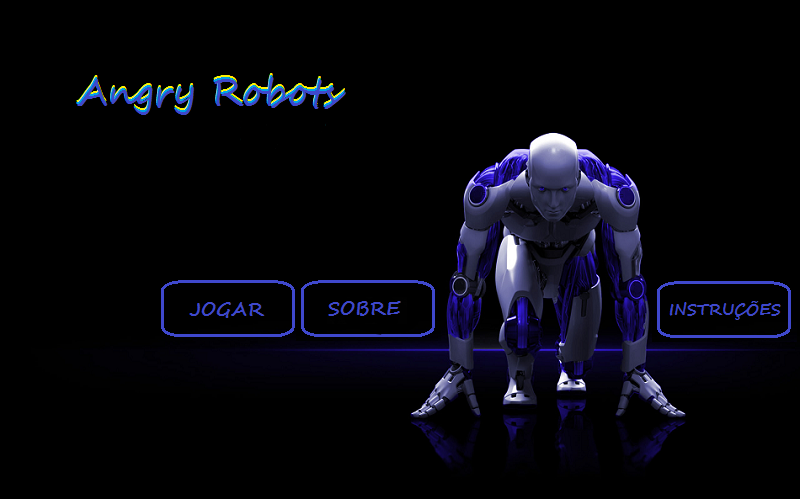
\includegraphics[scale=0.8]{menu.png}
\caption{Menu do jogo.}
\end{figure}

\section{Introducão}
\paragraph{}Nos últimos anos a industria de jogos cresceu de forma constante, e com ela a importância dos mesmos para o desenvolvimento de muitas habilidades humanas. Sabemos que a maioria dos jogos são desenvolvidos com intuito de estabelecer uma conexão entre o mundo virtual e o real, para que desta forma possa proporcionar ao jogador tanto uma diversão quanto o desenvolvimento de suas habilidade pessoais, como agilidades, raciocínio lógico, estratégia, entre outros, assim lhe ocasionando um exercício mental.
\paragraph{}Angry Robots, faz com que o jogador se movimente de forma rápida e lógica para que consiga chegar ao objetivo final, ganhar a partida e derrotar o robô.
\paragraph{}Em relação a visão computacional, quando tratada a imagem, utiliza-se algorítimos e fórmulas matemáticas, e principalmente a física, fundamental para calcular a frequência e tonalidade de cores, a iluminação e luminosidade do local, de maneira que possamos descobrir em qual escala de cor se encontra e melhorar a qualidade visual do jogo.

\begin{figure}[!htb]
\centering
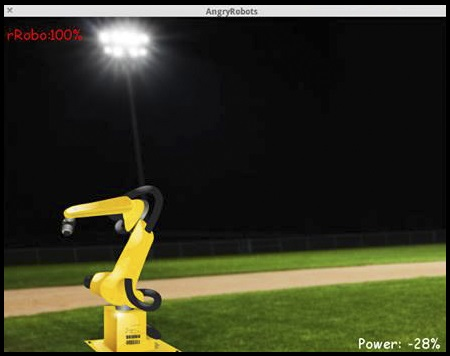
\includegraphics[scale=1.4]{betateste.jpg}
\caption{Versão beta do jogo, com design teste.}
\end{figure}

\vspace{0.7cm}

\newcommand{\imsize}{0.45\columnwidth}

\section{Revisão de Literatura}
\paragraph{}Angry Robots é um jogo limitado, pois dentro das exigências foram permitidos somente as bibliotecas, allegro 5 graficamente e a multiplataforma OpenCV utilizada para desenvolvimento de aplicativos na área de visão computacional.
\paragraph{}Existem diversos jogos em que o Angry Robots foi baseado, um deles foi o Cube Slam, um jogo em que os usuários se enfrentam numa partida visual de air hockey, no qual o jogador luta contra um urso, já no Angry Robots o adversário é um robô rápido e ágil.
\paragraph{}Há projetos no blog "Laboratório Garagem", entretanto todos fugiam do ambiente proposto, a maioria deles utilizavam Arduíno, OpenCV e Python. Porém, mesmo com os obstáculos impostos no Angry Robots, foi de grande utilidade pois algumas ideias surgiram através de post's referentes à robôs.
\paragraph{}Gran Slam Tennis 2, jogo que simula os grandes campeonatos de tênis, foi utilizado como base para os movimentos do jogo. 
\paragraph{}Os algorítimos desenvolvidos são autorais sem base em outros jogos, visto que mesmo com fundamento em tantos jogos, Angry Robots é um diferencial.

\section{Desenvolvimentos}

\textbf{Centróide} \\ \\ 
É o ponto interior que define seu centro geométrico, caso a forma geométrica represente uma secção homogênea de um corpo, então o centroide coincide com o centro de massa. A mesma foi implementada no Angry Robots para captar o meio da tela, facilitando a detecção e visualização do restante do display para uma variação é identificação da cor de preferência, no caso o azul.

\begin{figure}[!htb]
\centering
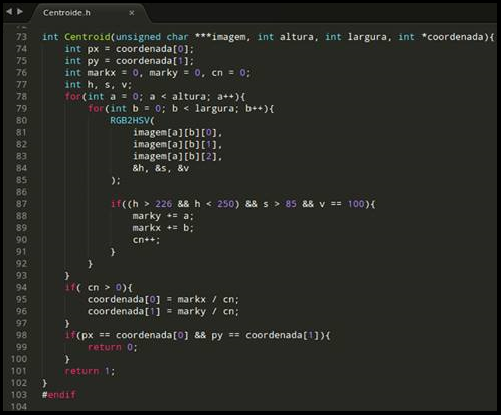
\includegraphics[scale=1.7]{centroid.png}
\caption{Exemplo: Código Centróide.}
\end{figure}

\textbf{Conversão para HSV} \\ \\
Calcula a intensidade da tonalidade, saturação e brilho da imagem, possibilitando aprimoramento no rastreamento do código, para resolver problemas com a iluminação do local, assim, não atrapalha a jogabilidade. A tonalidade permite distinguir as cores puras de 0 á 360 graus, a saturação verifica a intensidade da pureza da tonalidade, o brilho verifica a iluminação da imagem.

\begin{figure}[!htb]
\centering
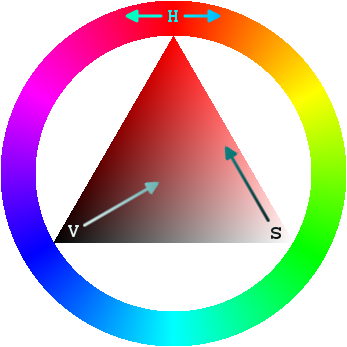
\includegraphics[scale=0.7]{Triangulo_HSV.png}
\caption{Exemplo: triangulo de explicação HSV }
\end{figure}

\textbf{Histograma} \\

Um histograma, conhecido também como distribuição de frequências. Aplicado no código para captar os tons de azul, onde todos os valores abaixo da media automaticamente são zerados e os maiores maximizados, para que se encaixem no tom rastreado, calculando assim o centro.

\begin{figure}[!htb]
\centering
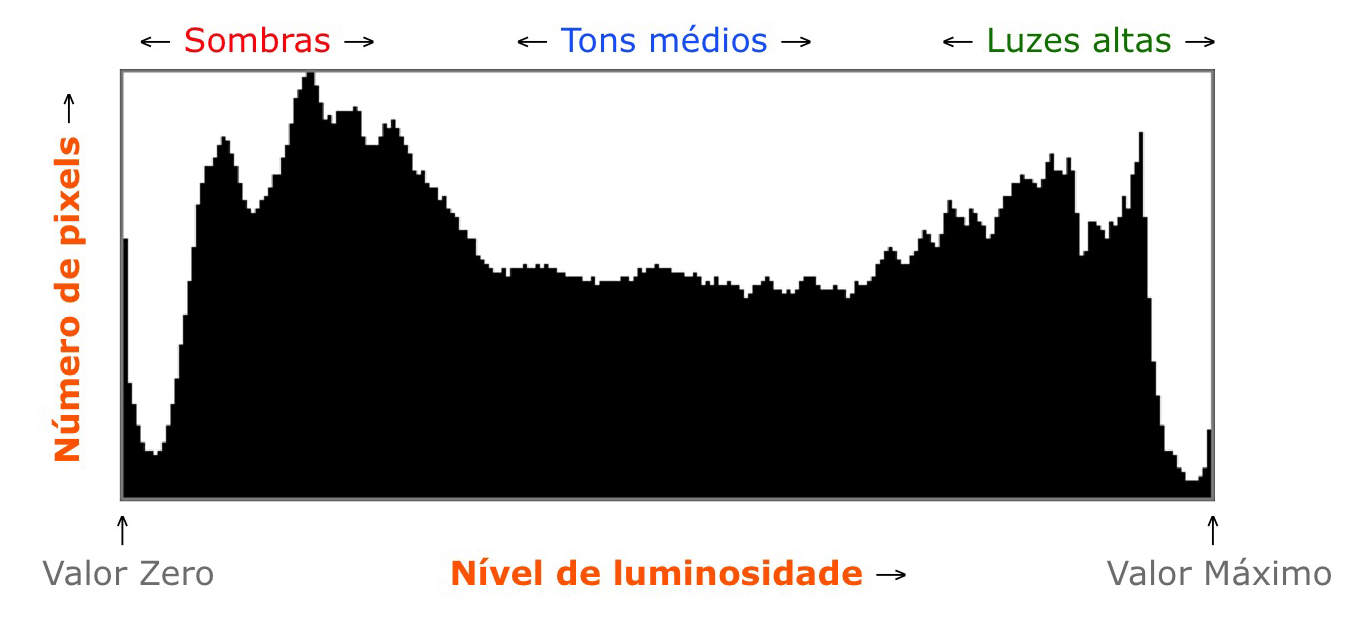
\includegraphics[scale=0.4]{histograma.jpg}
\caption{Exemplo: Nivél de frequência da cor.}
\end{figure}



\section{Resultados }

Neste jogo o robô ira tentar fugir para que o jogador não consiga acerta-lo com pequenas bolas, 
isto será feito através de um laser azul, o objetivo do jogo é derrotar o robô jogando as bolas em sua direção, quanto mais rápido os movimentos do usuário, mais chances de vencer o jogo.

\vspace{0.7cm}

\begin{figure}[!htb]
\centering

\includegraphics[scale=0.7]{fundo.jpg}
\caption{Imagem do jogo funcionando}
\end{figure}

\section{Considerações Finais}

O rastreamento é o ponto mais difícil, pois alguns fatores atrapalharam o desenvolvimento do mesmo, um deles foi a iluminação, pois devido a ela, a imagem pode ser ofuscada ou obscurecida demais, porém o HSV permitiu que a iluminação fosse ignorada, pois este algoritmo converte toda a imagem para cinza, e trata a variação da luminosidade, deste modo o usuário poderá jogar com uma camiseta azul por exemplo, sem afetar o rastreamento.


\bibliographystyle{plain}
\begin{thebibliography}{5}

\bibitem{site r7}  Portal R7 de notícias 
\\
\newblock http://noticias.r7.com/tecnologia-e-ciencia/noticias/jovens-apelam-para-games-corporais-para-melhorar-condicionamento-fisico-20110527.html

\bibitem{livro}
H. M. Deitel e P. J. Deitel.
\newblock Como programar em C, 2º edição.

\bibitem{site allegro} http://www.rafaeltoledo.net/tutoriais-allegro-5/
\\
\newblock Allegro 5.

\bibitem{site opencv} http://opencv.org/
\\
\newblock OpenCv

\bibitem{site rgb} http://www.rapidtables.com/web/color/RGB\_Color.htm \\
\newblock RGB

\end{thebibliography}

\end{multicols}

\end{document}

